% !TEX spellcheck = en_US
% !TEX spellcheck = LaTeX

\documentclass[letterpaper,10pt,english]{article}
\title{Lecture-29: Thermodynamics and Information Theory}
\author{}
\date{}
\usepackage{graphicx}
\usepackage{amsmath}
\usepackage{braket}
\usepackage{esvect}
\begin{document}

\maketitle
\section{Brief Overview of Thermodynamics}
\subsection{Classical Thermodynamics}
Thermodynamics is the branch of physics which deals with the flow of energy and its relationship with work and other measurable quantities. This field was formalized in the early 1800s, with the introduction of the laws of thermodynamics.
\subsubsection{Zeroth law of thermodynamics}
\textbf{Zeroth law of thermodynamics:} If two thermodynamic systems are each in thermal equilibrium with a third system, then they are in thermal equilibrium with each other. \\
This statement may seem trivial at first sight. The essence of the zeroth law is that there is a measurable quantity for every thermodynamic system, which we call temperature. The third system can be taken to be a thermometer, a device which measures the temperature of a system by reaching thermal equilibrium with it. By the zeroth law, the temperature of two systems are equal if and only if they are in thermodynamic equilibrium with each other. 
\subsubsection{First law of thermodynamics}
Investigations into the nature of work and energy came about when the first engines were invented. Scientists realized that the amount of heat absorbed/emitted by the engine and the amount of work performed by it are, in general, not functions of only the final and initial states of the engine. They depend on that path taken by the engine. However, the difference between the heat absorbed and the work done was a constant if the final and initial states were fixed. This quantity seemed to be a property of the system itself and not of the path taken, and thus, was labeled as the change in the internal energy of the system. Mathematically, we have:
\begin{equation*}
\Delta Q - \Delta W=\Delta U
\end{equation*}
or, in the infinitesimal limit, 
\begin{equation}
dQ=dW+dU
\end{equation}
Qualitatively, we may state this law as "in a thermodynamic process involving a closed system, the increment in the internal energy is equal to the difference between the heat accumulated by the system and the work done by it". However, heat and work are both forms of energy. So, we can state the first law as:\\
\textbf{First law of thermodynamics:} The total energy of an isolated system is a constant. Energy can neither be created nor destroyed, but can be transformed from one form to another. \\
\subsubsection{Second law of thermodynamics}
There are many processes that we can think of that would satisfy the first law, but do not occur in the natural world. For example, a body should be able to spontaneously cool down and elevate against gravity, but this obviously doesn't happen. The condition of a process to occur naturally or not is given by the second law, which has many different forms. \\
\textbf{Kelvin Statement:} It is impossible for any thermodynamic process to convert a quantity of heat entirely into work. \\
\textbf{Clausius Statement:} It is impossible for any thermodynamic process to transfer heat from a colder body to a hotter body as the sole result. \\
One can easy check that these statements are equivalent. \\
We can put the second law in the form of a mathematical statement:\\
\textbf{Clausius inequality:} for a system which undergoes a cyclic process by changing heat with external reservoirs, we must have:
\begin{equation}
\oint \frac{dQ}{T} \leq 0
\end{equation}
where, a cyclic process is defined as a process in which the initial and final states of the system are the same. The proof of this inequality is in Appendix A. \\
A reversible process is defined as a process whose direction can be reversed by producing infinitesimal changes in the system or the surroundings. It can run in both a "forward' or "backward" direction between the initial and final states. if we consider that the cyclic process in question is reversible, then the process characterized by $dQ \rightarrow -dQ$ must also be possible, so we have 
\begin{equation*}
\oint \frac{dQ}{T} \leq 0 \quad \text{ and } \quad \oint \frac{-dQ}{T} \leq 0
\end{equation*}
which implies that for a reversible process, 
\begin{equation}
\oint \frac{dQ_{rev}}{T} = 0
\end{equation}
Consider now, a reversible path which starts at state A and ends at state B, which we call as path 1. Suppose that there exists two distinct reversible paths which start from B and end at A, labeled path 2 and path 3. Obviously, path 1 + path 2 and path 1 + path 3 each form reversible cyclic processes. \\
For process path 1 + path 2, we have 
\begin{equation*}
\int_{1} \frac{dQ}{T} + \int_{2} \frac{dQ}{T}=0
\end{equation*}
whereas for the process path 1 + path 3, we have 
\begin{equation*}
\int_{1} \frac{dQ}{T} + \int_{3} \frac{dQ}{T}=0
\end{equation*}
which implies 
\begin{equation*}
\int_{2} \frac{dQ}{T} =\int_{3} \frac{dQ}{T}
\end{equation*}
This argument can be extended to any number of reversible paths between two states. Therefore, for a reversible process between final and initial states A and B, $\int_{A}^{B} \frac{dQ}{T}$ does not depend on the path chosen and depends only on A and B. Furthermore, if A=B, we must have the integral going to 0. Therefore, we can write 
\begin{equation}
\int_{A}^{B} \frac{dQ_{rev}}{T} =S(B)-S(A)
\end{equation}
where S(X) is the thermodynamic entropy of the system at state X. \\
If the path reversibly changes the state of a system by an infinitesimal amount from A to A+dA, we have:
\begin{equation*}
\int_{A}^{A+dA} \frac{dQ_{rev}}{T} =S(A+dA)-S(A) \rightarrow \frac{dQ_{rev}}{T}=dS
\end{equation*}
Note that for any general process, by the Clausius inequality, we have 
\begin{equation*}
\int_{A}^{B} \frac{dQ}{T} \leq S(B)-S(A) \quad \text{and } \quad \frac{dQ}{T} \leq dS
\end{equation*}
with equality if and only if the process is reversible. \\
An important result which we will use later is the entropy change during the isothermal heating of an ideal gas. The equation of state of one mole of an ideal gas is $PV=RT$. The work done is $PdV$. For isothermal heating, the internal energy of the gas doesn't change, so the heat change is equal to the work done. 
\begin{equation*}
\Delta S=\int \frac{dQ}{T}=\int \frac{PdV}{T}=\int \frac {(RT/V) dV}{T}=\int \frac{R dV}{V}
\end{equation*}
If the volume is changed from $V_1$ to $V_2$, we get 
\begin{equation*}
\Delta S=R \log \frac{V_2}{V_1}
\end{equation*}
If we have just a single particle, this equation becomes 
\begin{equation*}
\Delta S=k_B \log \frac{V_2}{V_1}
\end{equation*}
\subsection{Statistical Interpretation}
\subsubsection{Boltzman Entropy}
In the late 1800s, Ludwig Boltzmann gave the first statistical definition of entropy. First, we must define a couple of terms: \\
The \textbf{microstate} of a system is set of values of the position and momentum of each of its N particles. It forms a 6 dimensional subspace (each particle's position and momentum takes 3 variables each to represent). \\
The \textbf{macrostate} of a system is the specification of it in terms of its macroscopic properties, like pressure, temperature, volume, etc. \\
Therefore, we can think of the 6 dimensional phase space of a single particle partitioned into different cells, each corresponding to the microstate of the single particle. The microstate of the entire system consists of arranging N particles in the different cells of this single-particle microstate, which in turn determines the system's macrostate. \\
Boltzmann gave the formula for the entropy of a system:

\begin{equation}
S=k_B \log W
\end{equation}
where S is the entropy of the system, W is the number of microstates corresponding to a particular macrostate, and $k_B$ is a constant, equal to $1.38 \times 10^{-23}$ J/K. \\
If we have partitioned the single-particle microstate into k cells, then the number of microstates of an N-particle system corresponding to the same macrostate is simply the number of ways we can arrange N identical particles in k cells. \\
\begin{align*}
W&=\frac{N!}{n_1!n_2!\ldots n_k!} \quad \text{ with } \quad n_1+n_2+\ldots+n_k=N \\
S&=k_B \log W=k_b \left(\log(N!)-\log(n_1!)-\log(n_2!)-\ldots-\log(n_k!)\right)\\
& \approx k_B \left( (N \log N -N)-(n_1 \log n_1-n_1)-\ldots-(n_k \log n_k-n_k) \right) \\
&=-k_B\sum_i^k{n_i \log n_i}+const
\end{align*}
We can drop the constant, as it is really the entropy difference between two states that we care about. \\
Let $p_i=n_i/N$ be the probability of finding a random particle in the $i^{th}$ cell. Then, the expression for entropy reduces to:
\begin{equation}
S=-Nk_B\sum_i{p_i \log p_i}
\end{equation}
The entropy is a measure of how much we can infer about the arrangement of a system on the basis of its distribution. The higher the entropy, the less information that the distribution conveys about the arrangement of the system, and the more uncertainty and randomness there is. It can be shown that the distribution which maximises the entropy is given by 
\begin{equation}
n_i=\frac{e^{\beta E_i}}{\sum{e^{\beta E_i}}}
\end{equation}
where $E_i$ is the energy of the microstates in the $i^{th}$ call, and $\beta=1/k_B T$. The proof is given in Appendix B. This distribution is named the \textbf{Boltzmann distribution}. 
\subsubsection{Relation to thermodynamic entropy} 
We can show that if the probabilities are given by the Boltzmann distribution, the Boltzmann entropy reduces to the thermodynamic entropy. An infinitesimal change in entropy of one particle is given by 
\begin{align*}
dS&=-k_B \sum_i{dp_i \log p_i} \\
&=-k_B \sum_i{dp_i(-E_i/k_B T-ln Z)} \\
&=\sum_i {E_i dp_i/T} \quad \text{where we have used the conservation of probability, i.e.} \sum_i {dp_i=0} \\
&=\sum_i {\left( d(E_i p_i)-(dE_i)p_i\right)/T}
\end{align*}
Now, $\sum_i { d(E_i p_i)}$ is the expectation value of the change in the total energy of the system, $dU$. \\
If we are considering sufficiently slow changes so that the system remains in the same microscopic state, but the state itself changes slowly and reversibly, then  $\sum_i { (dE_i) p_i}$ is the expectation value of the total work done on the system by this reversible process, which by our sign convention, is $-dW_{rev}$. But by the first law of thermodynamics, we have $dU+dW_{rev}=dQ_{rev}$, so the entropy reduces to 
\begin{equation*}
dS=\frac{dQ_{rev}}{T}
\end{equation*}
which is exactly the thermodynamic entropy. 
\subsection{Free Energy}
The first law of thermodynamics states $\Delta Q=\Delta U+\Delta W$. Let us consider the work done when the system is transformed from an initial state A to a final state B under constant temperature. The second law thus gives:
\begin{equation*}
\int_A^B \frac{dQ}{T} \leq dS \rightarrow \Delta Q \leq T \left( S(B)-S(A) \right)
\end{equation*}
Therefore, we have 
\begin{equation*}
\Delta W \leq T\Delta S-\Delta U
\end{equation*}
Let us define a quantity $F=U-TS$. This gives us $\Delta W \leq -\Delta F$. Or, in other words, the word performed by an isothermal process is bounded above by the (negative of) the free energy change. \\
Consider now, a system which can exchange heat, but not work, with its surroundings. In that case, $\Delta W=0$, so we have $-\Delta F \geq 0$. If the system is transformed from state A to state B, we have $F(B) \leq F(A)$. So, we see that the free energy of an isolated system is always non-decreasing. The point of stable equilibrium corresponds to a minimum in free energy. 
\section{Information Theory} 
Information theory was born in 1948, when Claude Shannon published a paper entitled "A Mathematical Theory of Computation". He took they key approach that the entropy of a probability distribution is a measure of the information provided by it. 
\subsection{The Shannon Entropy}
Distributions with higher entropy have a larger amount of uncertainty involved in the outcome of a random process, so specifying its outcome will produce more information. \\
Shannon proposed a measure of information for X is a real valued function $H(X): {\text{ \{prob. distributions on X\} }} \rightarrow \mathcal{R}$ that satisfies:
\begin{itemize}
\item \textbf{Continuity:} $H(p_1, p_2, \ldots p_n)$ is continuous. 
\item \textbf{Monotonicity:} If the probability distribution is uniform, i.e. if $p_i=1/n$, then $H(1/n, \ldots 1/n)$ is a monotonic increasing function of n. 
\item \textbf{Composition law:} $H(X)$ is independent of how the process was broken into parts. This means that 
\begin{equation*}
H(PQ)=H(P)+\sum_i p_i H(Q \mid P)
\end{equation*}
\item \textbf{Normalization:} The information of a distribution with two equally likely events is 1, i.e. $H(0.5, 0.5)=1$. 
\end{itemize}
Then, there is one and only one function $H(X)$ which satisfies these conditions, and it is given by 
\begin{equation}
H(p_1 , \ldots , p_n)=-\sum_i {p_i \log_2 p_i}
\end{equation}
 The proof is in Appendix C. \\
There are several interpretations of the Shannon entropy. One interpretation, as we saw in class, is that $2^{NH(X)}$ is the number of typical messages with N letters. So, we can encode all these messages using only $NH(X)$ bits. Thus, H(X) represents the maximum amount that typical messages drawn from a  given set of letters can be compressed. \\
A second interpretation is that H(X) is a measure of the uncertainty of the probability distribution. The more certain a particular event is, the less information is associated with it. Thus, H(X) tells us our expected information gain upon measuring X. 
\subsection{Relationship between Shannon Entropy and Boltzmann Entropy}
We see that the Boltzmann entropy $S=-k_B \sum p_i \log p_i$ and the Shannon entropy $H=-\sum p_i \log_2 p_i$ look remarkably similar. They are equivalent up to a multiplicative constant of $k_B \log 2$. However, their physical significance are quite different. For example, if if we have a single transistor which is flipped to on or off with equal probability, the Shannon entropy of the transistor is 1 bit. However, the thermodynamic entropy of the transistor is exponentially higher. It counts each and every microstate which corresponds to a transistor being on or off, which is the configurations of all the atoms of the transistor. All this information of the billions of atoms of the transistor is not only unobtainable, but highly unnecessary. While it can be used to derive certain thermodynamic parameters of the transistor, the "real" information is just whether it is on or off. Thus, the Shannon entropy pertains to the amount of information of a system that we actually care about, like whether the transistor is on or off. It is a microscopic fraction of the Boltzmann entropy. \\
In a sense, the Shannon entropy is more fundamental than the Boltzmann entropy, as it is a quantity which can be attributed to any given probability distribution. If instead of just caring about if the transistor is on or off, our original question is about the states of each of the individual atoms, the Shannon entropy would be exactly equal to the Boltzmann entropy. This is the essence of \textbf{Landauer's principle}, which states that any information that has a physical representation must somehow be embedded in the statistical mechanical degrees of freedom of a physical or thermodynamic system. (We will encounter another form of Landauer's principle later.)
\subsection{Free Energy and Mutual Information}
Another interesting parallel is the relationship between free energy and mutual information. The second law states that the free energy of a system cannot increase spontaneously, whereas the data processing inequality gives us that the mutual information of two distributions cannot increase on a result of processing. \\
Let the two energy levels be $E_a$ and $E_b$, and their probabilities be $P_a(t)$ and $P_b(t)$. Note that we are not assuming that the probabilities are constant in time. The system's internal energy can therefore be represented as $U(\vec{P})=E_a P_a+E_b P_b=\vec{E}^{T} \vec{P}$, where $\vec{E}$ and $\vec{P}$ are column vectors. \\
The free energy is given by $F(\vec{P})=U(\vec{P})-TS(\vec{P})$. This can be rewritten as:
\begin{equation}
F(\vec{P})=\vec{E}^{T} \vec{P}- (k_B \log 2) T H(\vec{P})
\end{equation}
where $H(\vec{P})=-P_a \log_2 P_a -P_b \log_2 P_b$ is the Shannon entropy. \\
Now let's consider a seemingly unrelated problem: the transmission of a message over a noisy channel. At time $t=0$, a message is generated at the source, whose elements are drawn randomly and independently from $\vec{P}(0)$, which is a column vector of the $P_i (0)$'s. $P_i (0)$ is the probability of drawing the $i^{th}$ symbol. \\
If the transmission is through a noiseless channel, the message sent by the source and the message revieced by the receiver are the same. However, in a noisy channel, the message will get corrupted as it travels. If at $t=0$ the resident of some element of the message is i, then the probability that it will be corrupted into another symbol j after one time period is $T_{ji}$. Putting all the $T_{ji}$'s into a matrix $T$, we have:
\begin{equation*}
\vec{P}(1)=T \vec{P}(0)
\end{equation*}
After n time periods, we obviously have 
\begin{equation*}
\vec{P}(n)=T^n \vec{P}(0)
\end{equation*}
Information is lost when a message is trasmitted, because of the uncertainity aout what the identity of the element is upon reception. Therefore, we can define a quantity called \textbf{conditional entropy} as{
\begin{align*}
H(n \mid 0)=&H_a (n) P_a(0)+H_b(n) P_b (o)+ \ldots \\
=&\vec{H}^T (n) \vec{P}(0)
\end{align*}
where $\vec{H}^T (n)=\left( H(\text{column 1 of } T^n), H(\text{column 2 of } T^n), \ldots \right)$. Each component of $\vec{H}^T (n)$ is the entropy (information) lost during the transmission of that particular symbol. \\
In words, the conditional entropy is the sum of the entropies of the probability distributions which arise keeping the initial symbol fixed, multiplied by the probability of that initial symbol. It is a measyure of the information lost during transmission due to noise. \\
The difference in the information (entropy) supplied by the source and the information lost during transmission is the amount of information which survives through the transmission. This information (entropy) is mutually shared between the source and receiver. Therefore, we define the \textbf{mutual information} as:
\begin{equation}
I (\vec{P}(n), \vec{P}(0))=H(\vec{P}(n))-H(n \mid 0)=H(\vec{P}(n))-\vec{H}^T (n) \vec{P}(0)
\end{equation}
This looks rather similar to the equation for free energy, $F(\vec{P}(n))=\vec{E}^{T} \vec{P}(n)-(k_B \log 2) T  H(\vec{P}(n))$. In fact, we can make these equations look even similar by slightly manipulating them:
\begin{align*}
\frac{-F(\vec{P}(n))}{ k_B T \log 2 }=H(\vec{P}(n))-\frac{E^T}{ k_B T \log 2} \vec{P}(n) \\
I(\vec{P}(n))=H(\vec{P}(n)) - (H^T (n)) (T^{-n}) \vec{P}(n)
\end{align*}
We also have the data processing theorem, which states that the mutual information cannot increase on a result of processing. This is analogous to the fact that the free energy of a system cannot increase. \\
We know that the free energy is minimized when the distribution in question follows the Boltzmann distribution. Similarly, the mutual information will be maximized when the distribution follows a characteristic distribution for the channel, called the channel capacity distribution. This is the point of equilibrium of the source-receiver system, similar to the point of equilibrium of a thermodynamic system. 
\section{Information is Physical}
So far, the Shannon entropy and the concept of information are just mathematical constructs. In this section, we attempt to prove that information is something which exists in the physical world. 
\subsection{Maxwell's Demon}
Consider the setup shown below. A chamber is partitioned into two sides, and there is a microscopic valve in the partition that can be opened and closed with no expenditure of work. A gas with a high temperature is filled in side 1, and a gas with a lower temperature is filled in side 2. Note that this only means that the average energy of the gas molecules in side 1 is greater than the average energy of those in side 2. There will still be some molecules in side 1 with energy lower than the average energy in side 2 (called slow molecules), and there will still be some molecules in side 2 with energy higher than the average energy in side 1 (called fast molecules). \\
Maxwell's demon is a thought experiment, in which a demon (some supernatural agent) is able to measure the position and energy of each particle in the chamber and is able to open and close the valve so that only one molecule passes through. When he sees a slow molecule in side 1 approaching the valve, he opens it and allows the molecule to pass on to side 2. When he sees a fast molecule in side 2 approaching the valve, he opens it and allows the molecule to pass through. \\
After a some time, we see that the average energy of the molecules in side 1 will increase, while the average energy of the molecules in side 2 will decrease. Thus, there seems to be a transfer of energy from a colder temperature to a hotter temperature without the expenditure of work.  Moreover, the entropy of the system is decreased, even though it was an isolated system. This is in direct contradiction with the second law of thermodynamics. 
\subsection{Szilard's Engine}
Another apparent violation of the second law comes from Szilard's engine. Consider Maxwell's set-up, but with only a single gas particle in a box. If the supernatural demon knows which half of the box the particle is in (equivalent to a single bit of information), it can close a partition between the two halves of the box, close a piston unopposed into the empty half of the box, and then extract some amount of work by isothermally heating the gas. The particle can then be left to isothermally cool back to its original equilibrium occupied volume. Therefore, there is an apparent complete transfer of heat to work. Moreover, the entropy of the universe is decreased by $k_B \log 2$. 
\begin{figure}[h]
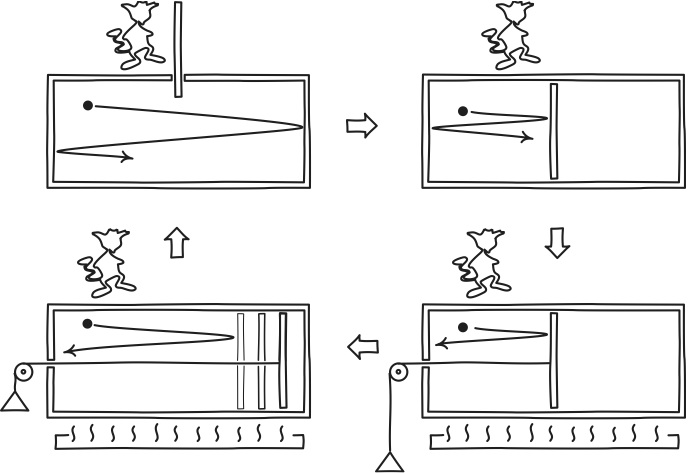
\includegraphics[width=\linewidth]{szilard.jpg}
\caption {Working of a Szilard engine}
\end{figure}
\subsection{Saving the Second Law}
The resolution of above paradoxes comes from the realization that in our original analysis, we considered the demon as some entity which just opens and closes the valve and does not interact with the system (the two gases) in any way. However, this is impossible, for the demon must also know when to open it, which means that it has some sort of sensor. The sensor will interact with the gas particles to determine its energy and position, and only then will the demon decide to open the valve. Thus, there is an interaction between the demon and the two gases, and so we must also consider the demon in our thermodynamic analysis. \\
In order to proceed further, we need to introduce two new principles: \\
\textbf{Szilard's Principle:} Gaining information that allows us to discern between n equally likely states is associated with a minimum increase in entropy of $k_B \log n$. \\
\textbf{Landauer's Principle:} Erasing information that allows us to discern between n equally likely states is associated with a minimum cost in entropy of $k_B \log n$. \\
The resolution of the Szilard engine comes from the fact that the entropy of the single particle system depends on the amount of information available to the observer. To the common man, the particle can be anywhere within the box. However, the demon already knows which half of the box the particle is in. This corresponds to him obtaining one bit of information (which half the particle is in). This results in a minimum entropy increase of $k_B \log 2$. Therefore, the decrease in entropy of the particle is countered by the increase in the entropy of the demon. When the engine is returned to its original state by isothermal cooling, the demon must destroy the one bit of information that he has. This is an irreversible process, which means that some amount of heat will be dissipated out by the demon. Thus, there is no complete conversion of heat to work. \\


In the first scenario, the demon must gain information of each of the particle's position, velocity, and energy in order to determine when to open the valve. This means that there is an increase in the entropy of the demon, which in turn means that the demon will heat up. This can be attributed as the the work done by the demon in order to sense and store the information of the particles. It turns out that the increase in the demon's entropy is at least as large as the decrease in entropy of the gas chambers. In addition, the heat gained by the demon is at least as large as the total energy transferred to from the hot gas to the cold gas. This is only a qualitative explanation.
\section{Topics of Current Research}
In this last section, we give an extremely brief overview of some of the present topics of research, where physics and information theory come together. 
\subsection{Quantum Computation}
In classical information theory, the state of a 2-bit system is \textbf{either 0 or 1}. In quantum information theory, however, it is impossible for us to tell beforehand what the state of the system is. it is therefore necessary to take a linear combination of the 0 and 1 states. Thus, a general quantum bit, or \textbf{qubit}, can be represented as: 
\begin{equation}
\ket{Q}=a\ket{0} +b\ket{1}
\end{equation}
where $|a|^2$ is the probability that the system is in state $\ket{0}$, and $|b|^2$ is the probability that the system is in state $\ket{1}$. We must have $|a|^2+|b|^2=1$. This resembles the equation of a circle. \\
Therefore, $\ket{Q}$ has no deterministic value before measuring. After measuring, however, it becomes determinate (either 0 or 1). We say that the act of measuring $\ket{Q}$ collapses its either $\ket{0}$ or $\ket{1}$. \\
A qubit encodes an arbitrarily large amount of information in the values of $a$ and $b$. However, the outcome of a measurement collapses its state to just one classical bit. Therefore, we say that a qubit encodes an arbitrarily large amount of information, but only one classical bit of it is available to us. \\
A qubit can be transformed from one state to another by means of linear transformations. However, a very key properties of qubits is that a quibit can neither be copied nor destroyed. This called the no-cloning theorem and the no-deleting theorem respectively. 
\subsection{Black Holes and Information}
For our purpose, we may take a black hole to be a body with a characteristic radius, called the event horizon, such that nothing can escape out of it. Therefore, any information which crosses the event horizon is lost to us. The loss of information from us means that the entropy of the rest of the universe decreases. Therefore, the only explanation is that the entropy of the black hole must increase. The Einstein field equations of general relativity gives us 
\begin{equation}
dA \left( \frac{c^4}{8 \pi G \left( r_H +\frac{GM}{c^2}+\frac{G^2 M^2}{c^4 r_H -c^2GM}\right)}\right)=d(Mc^2)-M\Omega dJ
\end{equation}
where $r_H$ is the radius of the event horizon, A is the area of the event horizon, M is the mass of the black hole, J is its specific angular momentum, and $\Omega$ is its angular velocity. $Mc^2$ can be considered as the internal energy of the black hole, and $M\Omega J$ is the work done in changing its angular momentum. Comparing with the first law of thermodynamics $TdS=dU+dW$, we see that the area of the event horizon is a measure of the entropy of the black hole. Furthermore, general relativistic calculations show that $A \propto M^2$. Therefore, if a body falls inside the black hole, the area of the black hole increases, which shows that its entropy increases. \\
In 1974, Stephen Hawking united quantum field theory and general relativity to show that, over immensely long time scales, a black hole emits radiation. The source of this radiation, now known as Hawking radiation, is the mass of the black hole itself. As Hawking radiation is emitted, the mass of the black hole must therefore decrease, which reduces its entropy. Furthermore, the nature of the radiation follows a black body spectrum, with temperature given by 
\begin{equation}
T=\frac{\hbar c^3}{8 \pi G k_B M}
\end{equation}
This spectrum is completely independent of what the black hole is made of. Essentially, any information that fell into the black hole is lost from the universe when it is emitted as Hawking radiation. \\
The black hole information paradox is one of the biggest puzzles of modern physics. There have been many attempts to resolve it, including but not limited to, creation of separate baby-universes, leaking out of information from the black hole, and the acceptance that the information is irretrievably lost. However, that is a story for another lecture!
\begin{thebibliography}{99}
\bibitem{1} Shannon, C.E. "A Mathematical Theory of Communication". The Bell System Technical Journal, Vol. 27. October, 1948.
\bibitem{2} Jaynes, E.T. "Information Theory and Statistical Mechanics". The Physical Review, Vol. 106. May, 1957
\bibitem{3} Kafri, Oded. "The Second Law and Informatics". Varicom Communications. Isreal, Tel Aviv.
\bibitem{4} Feinstein, David. "Relating Thermodynamics to Information Theory: The Equality of Free Energy and Mutual Information". California Institute of Technology, 1986. 
\bibitem{5} K. Huang, "Statistical Mechanics", John Wiely, New York. 1987. 
\end{thebibliography}
\section*{Appendices} 
\subsection*{Appendix A: Proof of Clausius Inequality}
In order to prove this, we must first define what a \textbf{Carnot engine} is. It is a reversible heat engine which uses an ideal gas and works between a hot reservoir at temperature $T_H$ and a cold reservoir at temperature $T_C$. The working consists of four steps:
\begin{itemize}
\item Isothermal expansion of the gas at $T_H$
\item Adiabatic expansion of the gas from $T_H$ to $T_C$
\item Isothermal compression of the gas at $T_C$
\item Adiabatic compression of the gas from $T_C$ to $T_H$
\end{itemize}
The net result of the process is absorption of heat $Q_H$ from the hot reservoir, rejection of heat $Q_C$ to the cold reservoir, and extraction of work $Q_H-Q_C$. It can be easily shown that $\frac{Q_C}{Q_H}=\frac{T_C}{T_H}$. \\
Now, onto the Clausius inequality. Let the cyclic transformation be divided into n infinitesimal steps for which the temperature may be considered to be a constant in each step. The system is imagined to be brought successively into contact with heat reservoirs at temperatures $T_1$, $T_2$, ..., $T_n$. Let the amount of heat absorbed by the system during the $i$th step from the heat reservoir be $Q_i$. If we prove that $\sum_{i=1}^{n} \frac{Q_i}{T_i} \leq 0$, then the Claussius inequality is obtained as $n\rightarrow \infty$. \\
Construct a set of n Carnot engines ${C_1, C_2, \ldots, C_n}$ such that $C_i$:
\begin{itemize}
\item operates between $T_i$ and $T_0$ ($T_0 \geq T_i$ for all i)
\item absorbs heat $Q_i^0$ from $T_0$. 
\item rejects $Q_i$ to $T_i$. 
\end{itemize} 
Therefore, we have $\frac{Q_i^0}{Q_i}=\frac{T_0}{T_i}$
Consider the operation consisting of the cyclic process plus ${C_1+ C_2+ \ldots+ C_n}$. The net result of this cycle is that an amount of heat 
\begin{equation*}
Q_0=\sum_{i=1}^{n} Q_i^0=T_0\sum_{i=1}^{n} \frac{Q_i}{T_i}
\end{equation*}
is absorbed from the reservoir $T_0$ and converted entirely into work, with no other effect. According to the second law, this is impossible unless $Q_0 \leq 0$. Therefore, we have 
\begin{equation*}
\sum_{i=1}^{n} \frac{Q_i}{T_i} \leq 0
\end{equation*}
Taking the limit $n\rightarrow \infty$ gives us the Clausius inequality. 
\subsection*{Appendix B: The Boltzmann Distribution}
We find the probability distribution which maximises the Boltzmann entropy by the method of Lagrangian multipliers. We have $dS=-k_B \sum \log n dn=0$ (replace $p_i$ by $n_i$), subject to two constraints:
\begin{itemize}
\item The total number of particles is constant. Therefore, we have $N=\sum n_i$ and $dN=\sum dn_i=0$.
\item There is no change in the total energy of the system. $U=\sum E_i n_i$ and $dU=\sum E_i dn_i =0$. 
\end{itemize}
Letting $\alpha$ and $\beta$ be our Lagrangian multipliers, we have:
\begin{align*}
dS=&\sum(-k_B \log n +\alpha +\beta E_i)dn_i=0 \\
&-k_B \log n +\alpha +\beta E_i=0 \\
n^{*}_i=&e^{(\alpha+\beta E_i)/k} \quad \text{as the solution}
\end{align*}
Substituting this value of $n_i^{*}$ in the constraint, we have $N=\sum e^{(\alpha+\beta E_i)/k_B}=e^{\alpha/k_B}\sum e^{\beta E_i/k_B}$. Therefore, 
\begin{equation*}
\alpha=k_B \log(N/\sum e^{\beta E_i/k_B})
\end{equation*}
We procede further by: 
\begin{align*}
dS(n_i^{*})=&-k_B \sum log n_i^{*} dn_i \\
=& -k_B \sum (\alpha+\beta E_i)/k dn_i \\
=& -\beta \sum E_i dn_i \\
=& -\beta dQ
\end{align*}
Comparing with $dS=dQ/T$, we get $\beta=-1/T$. This gives the Boltzmann distribution. 
\subsection*{Appendix C: The Shannon Entropy}
To show that the Shannon entropy is the only function that satisfies all the three conditions listed, we design a special compound experiment. \\
Consider an experiment in which we randomly pick one object out of N objects. The probability of picking any onjext is $1/N$ Therefore, the entropy of the experiment is 
\begin{equation*}
H(1/N, 1/N, \ldots, 1/N) =f(N)
\end{equation*}
Now, we divide the N objects into m groups. Each group k contains $n_k$ objects. Obviously, $\sum_{k_1}^{m} n_k=N$. The experiment is now performed in two steps. In the first step, we randomly rick one of the m groups, and in the second step, we pick one object from the selected group. \\
Let the probability of selecting the $k^{th}$ group be $p_k$. The probability of selecting any object in the $k^{th}$ group is $1/n_k$. Since the total information or entropy must be the same, we have
\begin{equation*}
f(N)=H(p_1, \ldots, p_m)+\sum_{k=1}^{m} p_k f(n_k)
\end{equation*}
Now, consider the case in which all the groups have equal objects. Therefore, $n_1=n_2=\ldots=n_m=n=N/m$ and $p_k=1/m$ for all k. 
\begin{align*}
f(N)=H(1/m, \ldots ,1/m) +\sum_{k=1}^{m} \frac{1}{m}f(n) \\
f(nm)=f(m)+f(n) \text{ for arbitrary m and n} \\
\Rightarrow f(m)=K \log m
\end{align*}
where K is an arbitrary constant. \\
Now, plug this back to the general case. 
\begin{align*}
K \log N=&H(p_1, \ldots , p_m) +K\sum p_k \log n_k \\
H(p_1, \ldots, p_m)=&K \log N-k\sum p_k \log n_k \\
=&K \sum p_k \log N -K\sum p_k \log n_k \\
=& K\sum p_k \log \frac{N}{n_k} \\
=&-K\sum p_k \log p_k
\end{align*}
When we impose the last normalization condition, we get the value of K to be $\frac{1}{\log 2}$. Therefore, the only function which satisfies all the conditions is 
\begin{equation*}
H(p_1, \ldots p_m)=-\sum p_i \log_2 p_i
\end{equation*}
\end{document}